% Candidate source: src-2323f00197bbd8d5c8353a847fc0e7ccfc52169ca219272ee58990ae4b6ecba3
% Source PDF SHA-256: be2accb36a086126db90ee7c5a217e08e55429053a4167df1ad58bbfb213de46
% PDF page 1 (printed page 180), question 15.
% Redraw follows visible/hidden edges; oblique quadrangular prism ABCD-A1B1C1D1.
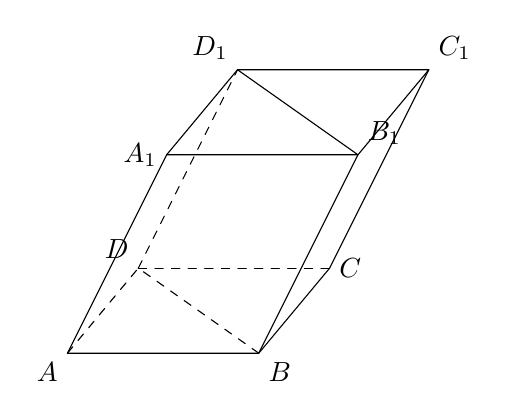
\begin{tikzpicture}[line cap=round,line join=round,>=latex,x=0.9cm,y=0.9cm]
  % Base vertices
  \coordinate (A) at (-1.5,-1.2);
  \coordinate (B) at (1.2,-1.2);
  \coordinate (C) at (2.2,0);
  \coordinate (D) at (-0.5,0);

  % Top vertices shifted by (1.4, 2.8)
  \coordinate (A1) at (-0.1,1.6);
  \coordinate (B1) at (2.6,1.6);
  \coordinate (C1) at (3.6,2.8);
  \coordinate (D1) at (0.9,2.8);

  % Hidden edges
  \draw[dashed] (A) -- (D);
  \draw[dashed] (D) -- (C);
  \draw[dashed] (D) -- (D1);
  \draw[dashed] (B) -- (D);

  % Visible edges: base
  \draw (A) -- (B) -- (C);

  % Visible edges: lateral
  \draw (A) -- (A1);
  \draw (B) -- (B1);
  \draw (C) -- (C1);

  % Visible edges: top
  \draw (A1) -- (B1) -- (C1) -- (D1) -- cycle;

  % Diagonal on top face
  \draw (B1) -- (D1);

  % Labels
  \node[below left] at (A) {$A$};
  \node[below right] at (B) {$B$};
  \node[right] at (C) {$C$};
  \node[above left] at (D) {$D$};
  \node[left] at (A1) {$A_1$};
  \node[above right] at (B1) {$B_1$};
  \node[above right] at (C1) {$C_1$};
  \node[above left] at (D1) {$D_1$};
\end{tikzpicture}
